% meta.concepts: 2D equivalent systems
% meta.tags: test concept
% acknowledge: Peter Seiler graciously Fall 2013 course material
% source: 2013 P. Seiler AEM2011 Exam 1

\noindent The bar shown in Figure~\ref{fig:Orig} below has forces acting at various points on the right and one couple of
magnitude $10 N \cdot m$ acting on the left.  Under this loading, the bar is in static equilbrium.

 \begin{figure}[ht!]
    \centering
    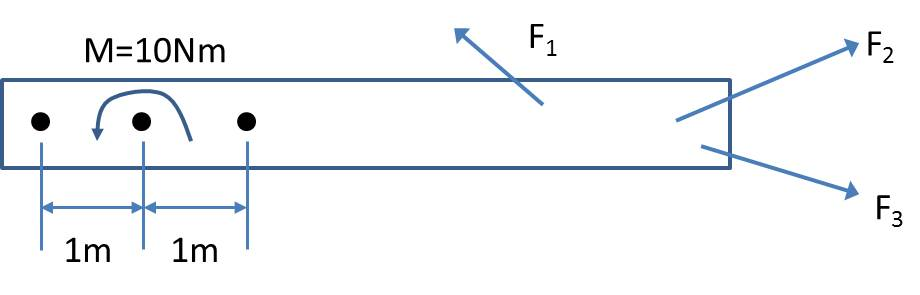
\includegraphics[width=3in]{BarOriginal.jpg}
    \caption{Bar in static equilibrium}
    \label{fig:Orig}
  \end{figure}

\noindent For each of the following modified loads, will the bar still maintain static equilibrium?  Briefly justify your answer for each case.
  \begin{figure}[ht!]
    \centering
    \subfigure[]{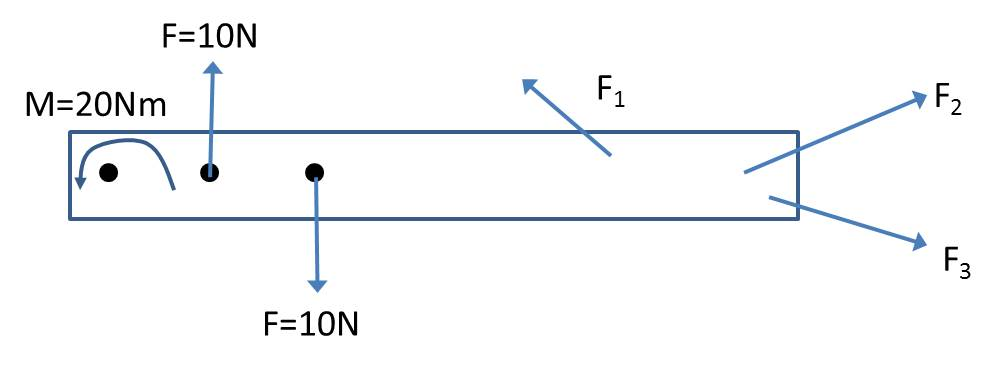
\includegraphics[width=3in]{BarA.jpg}} \qquad
    \subfigure[]{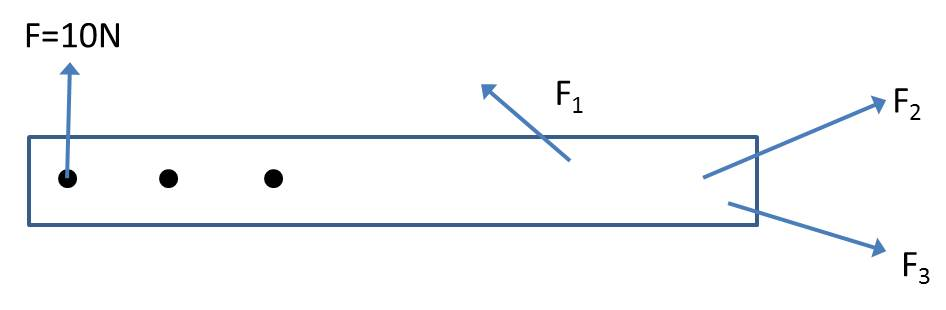
\includegraphics[width=3in]{BarB.jpg}}
  \end{figure}
  \begin{figure}[ht!]
    \centering
    \subfigure[]{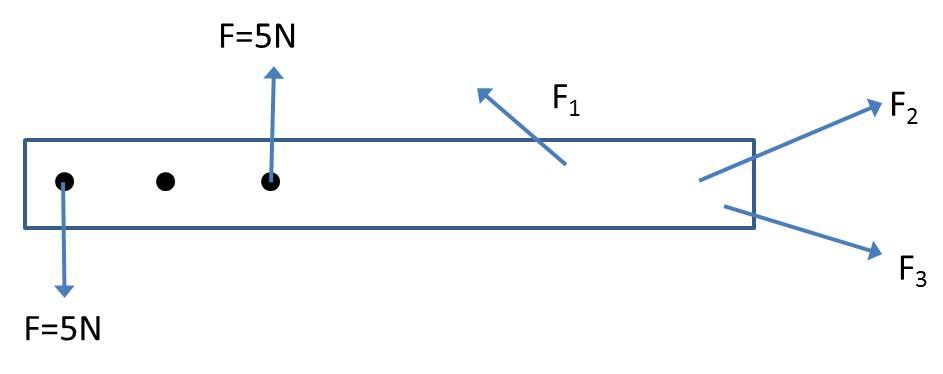
\includegraphics[width=3in]{BarC.jpg}} \qquad
    \subfigure[]{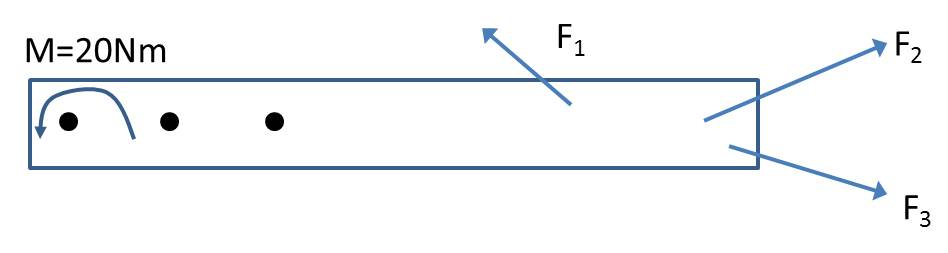
\includegraphics[width=3in]{BarD.jpg}}
  \end{figure}
  \begin{figure}[ht!]
    \centering
    \subfigure[]{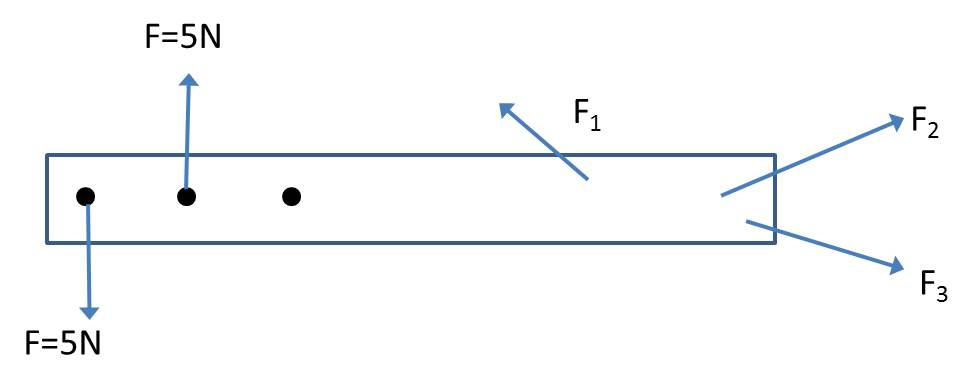
\includegraphics[width=3in]{BarE.jpg}} \qquad
    \subfigure[]{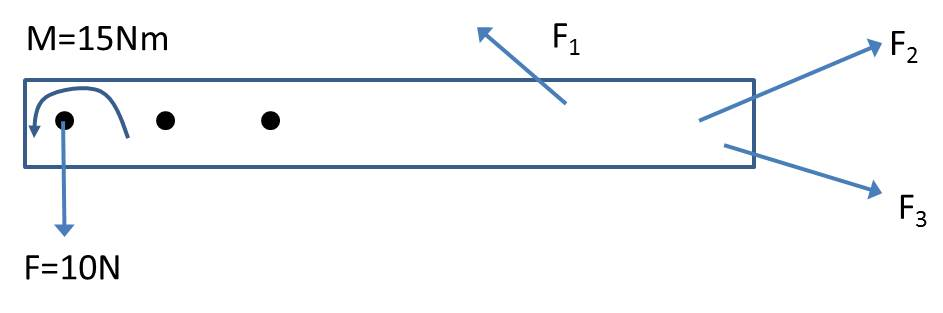
\includegraphics[width=3in]{BarF.jpg}}
  \end{figure}







































